\PassOptionsToPackage{unicode=true}{hyperref} % options for packages loaded elsewhere
\PassOptionsToPackage{hyphens}{url}
%
\documentclass[]{article}
\usepackage{lmodern}
\usepackage{amssymb,amsmath}
\usepackage{ifxetex,ifluatex}
\usepackage{fixltx2e} % provides \textsubscript
\ifnum 0\ifxetex 1\fi\ifluatex 1\fi=0 % if pdftex
  \usepackage[T1]{fontenc}
  \usepackage[utf8]{inputenc}
  \usepackage{textcomp} % provides euro and other symbols
\else % if luatex or xelatex
  \usepackage{unicode-math}
  \defaultfontfeatures{Ligatures=TeX,Scale=MatchLowercase}
\fi
% use upquote if available, for straight quotes in verbatim environments
\IfFileExists{upquote.sty}{\usepackage{upquote}}{}
% use microtype if available
\IfFileExists{microtype.sty}{%
\usepackage[]{microtype}
\UseMicrotypeSet[protrusion]{basicmath} % disable protrusion for tt fonts
}{}
\IfFileExists{parskip.sty}{%
\usepackage{parskip}
}{% else
\setlength{\parindent}{0pt}
\setlength{\parskip}{6pt plus 2pt minus 1pt}
}
\usepackage{hyperref}
\hypersetup{
            pdfborder={0 0 0},
            breaklinks=true}
\urlstyle{same}  % don't use monospace font for urls
\usepackage{color}
\usepackage{fancyvrb}
\newcommand{\VerbBar}{|}
\newcommand{\VERB}{\Verb[commandchars=\\\{\}]}
\DefineVerbatimEnvironment{Highlighting}{Verbatim}{commandchars=\\\{\}}
% Add ',fontsize=\small' for more characters per line
\newenvironment{Shaded}{}{}
\newcommand{\AlertTok}[1]{\textcolor[rgb]{1.00,0.00,0.00}{\textbf{#1}}}
\newcommand{\AnnotationTok}[1]{\textcolor[rgb]{0.38,0.63,0.69}{\textbf{\textit{#1}}}}
\newcommand{\AttributeTok}[1]{\textcolor[rgb]{0.49,0.56,0.16}{#1}}
\newcommand{\BaseNTok}[1]{\textcolor[rgb]{0.25,0.63,0.44}{#1}}
\newcommand{\BuiltInTok}[1]{#1}
\newcommand{\CharTok}[1]{\textcolor[rgb]{0.25,0.44,0.63}{#1}}
\newcommand{\CommentTok}[1]{\textcolor[rgb]{0.38,0.63,0.69}{\textit{#1}}}
\newcommand{\CommentVarTok}[1]{\textcolor[rgb]{0.38,0.63,0.69}{\textbf{\textit{#1}}}}
\newcommand{\ConstantTok}[1]{\textcolor[rgb]{0.53,0.00,0.00}{#1}}
\newcommand{\ControlFlowTok}[1]{\textcolor[rgb]{0.00,0.44,0.13}{\textbf{#1}}}
\newcommand{\DataTypeTok}[1]{\textcolor[rgb]{0.56,0.13,0.00}{#1}}
\newcommand{\DecValTok}[1]{\textcolor[rgb]{0.25,0.63,0.44}{#1}}
\newcommand{\DocumentationTok}[1]{\textcolor[rgb]{0.73,0.13,0.13}{\textit{#1}}}
\newcommand{\ErrorTok}[1]{\textcolor[rgb]{1.00,0.00,0.00}{\textbf{#1}}}
\newcommand{\ExtensionTok}[1]{#1}
\newcommand{\FloatTok}[1]{\textcolor[rgb]{0.25,0.63,0.44}{#1}}
\newcommand{\FunctionTok}[1]{\textcolor[rgb]{0.02,0.16,0.49}{#1}}
\newcommand{\ImportTok}[1]{#1}
\newcommand{\InformationTok}[1]{\textcolor[rgb]{0.38,0.63,0.69}{\textbf{\textit{#1}}}}
\newcommand{\KeywordTok}[1]{\textcolor[rgb]{0.00,0.44,0.13}{\textbf{#1}}}
\newcommand{\NormalTok}[1]{#1}
\newcommand{\OperatorTok}[1]{\textcolor[rgb]{0.40,0.40,0.40}{#1}}
\newcommand{\OtherTok}[1]{\textcolor[rgb]{0.00,0.44,0.13}{#1}}
\newcommand{\PreprocessorTok}[1]{\textcolor[rgb]{0.74,0.48,0.00}{#1}}
\newcommand{\RegionMarkerTok}[1]{#1}
\newcommand{\SpecialCharTok}[1]{\textcolor[rgb]{0.25,0.44,0.63}{#1}}
\newcommand{\SpecialStringTok}[1]{\textcolor[rgb]{0.73,0.40,0.53}{#1}}
\newcommand{\StringTok}[1]{\textcolor[rgb]{0.25,0.44,0.63}{#1}}
\newcommand{\VariableTok}[1]{\textcolor[rgb]{0.10,0.09,0.49}{#1}}
\newcommand{\VerbatimStringTok}[1]{\textcolor[rgb]{0.25,0.44,0.63}{#1}}
\newcommand{\WarningTok}[1]{\textcolor[rgb]{0.38,0.63,0.69}{\textbf{\textit{#1}}}}
\usepackage{graphicx,grffile}
\makeatletter
\def\maxwidth{\ifdim\Gin@nat@width>\linewidth\linewidth\else\Gin@nat@width\fi}
\def\maxheight{\ifdim\Gin@nat@height>\textheight\textheight\else\Gin@nat@height\fi}
\makeatother
% Scale images if necessary, so that they will not overflow the page
% margins by default, and it is still possible to overwrite the defaults
% using explicit options in \includegraphics[width, height, ...]{}
\setkeys{Gin}{width=\maxwidth,height=\maxheight,keepaspectratio}
\setlength{\emergencystretch}{3em}  % prevent overfull lines
\providecommand{\tightlist}{%
  \setlength{\itemsep}{0pt}\setlength{\parskip}{0pt}}
\setcounter{secnumdepth}{0}
% Redefines (sub)paragraphs to behave more like sections
\ifx\paragraph\undefined\else
\let\oldparagraph\paragraph
\renewcommand{\paragraph}[1]{\oldparagraph{#1}\mbox{}}
\fi
\ifx\subparagraph\undefined\else
\let\oldsubparagraph\subparagraph
\renewcommand{\subparagraph}[1]{\oldsubparagraph{#1}\mbox{}}
\fi

% set default figure placement to htbp
\makeatletter
\def\fps@figure{htbp}
\makeatother


\date{}

\begin{document}

\hypertarget{header-n1145}{%
\section{第三章 处理图像的颜色}\label{header-n1145}}

In this chapter, we will cover the following recipes:

\begin{itemize}
\item
  \protect\hyperlink{ch3_sdp}{Comparing colors using the Strategy design
  pattern使用策略设计模式比较颜色}
\item
  \protect\hyperlink{ch3_grabcut}{Segmenting an image with the GrabCut
  algorithm使用GrabCut算法分割图像}
\item
  \protect\hyperlink{ch3_ccr}{Converting color
  representations转换颜色表示}
\item
  \protect\hyperlink{ch3_hsb}{Representing colors with hue, saturation,
  and brightness 用色调,饱和度和亮度表示颜色}
\end{itemize}

\hypertarget{header-n1157}{%
\subsection{简介}\label{header-n1157}}

The ability to see the world in colors is one of the important
characteristics of the human visual system.The retina({[}ret·i·na
\textbar{}\textbar{} 'retɪnə{]}n. 视网膜) of the human eye includes
specialized photoreceptors({[}ˌfəutəuriˈseptə{]} 光感受器; 光敏接收器件;
光受器; 感光器; 感光受器), called cones({[}kəʊn{]}n. 圆锥体, 球果v.
使成锥形。这里翻译成"视锥细胞"), which are responsible for the
perception({[}per·cep·tion \textbar{}\textbar{} pər'sepʃn /pə'-{]}n.
知觉, 领悟力, 感觉) of colors. There are three types of cones that
differ in the wavelength range of light they absorb({[}ab·sorb
\textbar{}\textbar{} əb'sɔːb{]}v. 吸收; 使全神贯注; 汲取, 理解); using
the stimuli({[}'stim·u·lus \textbar{}\textbar{} stɪmjələs /-mjʊl-{]}n.
刺激, 刺激品, 激励) from these different cells, the human brain is able
to create color perception. Most other animals only have rod({[}rɑd
/rɒd{]}n. 竿, 小枝, 笞鞭) cells, which are photoreceptors with better
light sensitivity but that cover the full spectrum of visible light
without color discrimination. In the human eye, rods are mainly located
at the periphery of the retina, while the cones are concentrated in the
central part.

用颜色看世界的能力是人类视觉系统的重要特征之一。人眼的视网膜包括专门的光感受器,称为视锥细胞,负责感知颜色。有三种类型的锥体在它们吸收的光的波长范围内不同;利用来自这些不同细胞的刺激,人类的大脑能够产生色彩感知。大多数其他动物只有杆细胞,它们是光感受器,具有更好的光敏感性,但覆盖了全部可见光,没有颜色辨别。在人眼中,杆主要位于视网膜的周边,而锥体集中在视网膜的中央部分。

In digital imaging, colors are generally reproduced by using the red,
green, and blue additive({[}ad·di·tive \textbar{}\textbar{} 'ædɪtɪv{]}n.
添加剂; 添加物; 加法) primary colors.These have been selected because
when they are combined together, they can produce a wide
gamut({[}'gæmәt{]} n. 音阶, 整个范围, 全部, 音域) of different colors.
In fact, this choice of primaries mimics well the trichromatic color
perception of the human visual system as the different cone cells have
sensitivity located around the red, green, and blue spectrum. In this
chapter,you will play with the pixel color and see how an image can be
segmented based on the color information. In addition, you will learn
that it can sometimes be useful to use a different color representation
when performing color image processing.

在数字成像中,通常使用红色,绿色和蓝色这几种原色组合再现颜色。选择这些颜色是因为当它们组合在一起时,它们可以产生不同颜色的宽色域。实际上,这种原色的选择很好地模拟了人类视觉系统的三色颜色感知,因为不同的锥形细胞具有位于红色,绿色和蓝色光谱周围的灵敏度。在本章中,您将使用像素颜色,并查看如何根据颜色信息分割图像。此外,您将了解在执行彩色图像处理时使用不同的颜色表示有时会很有用。

\hypertarget{header-n1162}{%
\subsection{使用策略设计模式比较颜色}\label{header-n1162}}

Let's say we want to build a simple algorithm that will identify all of
the pixels in an image that have a given color. For this, the algorithm
has to accept an image and a color as input and will return a binary
image showing the pixels that have the specified color. The tolerance
with which we want to accept a color will be another parameter to be
specified before running the algorithm.

假设我们想要构建一个简单的算法来识别图像中具有给定颜色的所有像素。为此,算法必须接受图像和颜色作为输入,并返回显示具有指定颜色的像素的二进制图像。我们想要接受颜色的容差将是在运行算法之前指定的另一个参数。

In order to accomplish this objective, this recipe will use the Strategy
design pattern. This object-oriented design pattern constitutes an
excellent way of encapsulating an algorithm in a class. It becomes then
easier to replace a given algorithm with another one, or to chain
several algorithms together in order to build a more complex process. In
addition, this pattern facilitates the deployment of an algorithm by
hiding as much of its complexity as possible behind an intuitive
programming interface.

为了实现这一目标,该配方将使用策略设计模式。这种面向对象的设计模式构成了将算法封装在类中的极好方法。然后更容易用另一个算法替换给定的算法,或者将几个算法链接在一起以构建更复杂的过程。此外,该模式通过在直观的编程接口后面隐藏尽可能多的复杂性来促进算法的部署。

\hypertarget{header-n1167}{%
\subsubsection{How to do it\ldots{}}\label{header-n1167}}

Once an algorithm has been encapsulated in a class using the Strategy
design pattern, it can be deployed by creating an instance of this
class. Typically, the instance will be created when the program is
initialized.At the time of construction, the class instance will
initialize the different parameters of the algorithm with their default
values so that it will immediately be ready to be used. The algorithm's
parameter values can also be read and set using appropriate methods. In
the case of an application with a GUI, these parameters can be displayed
and modified using different widgets (text fields, sliders, and so on)
so that a user can easily play with them.

使用策略设计模式将算法封装在类中后,可以通过创建此类的实例来部署它。通常,在初始化程序时将创建实例。在构造时,类实例将使用其默认值初始化算法的不同参数,以便立即准备好使用它。也可以使用适当的方法读取和设置算法的参数值。对于具有GUI的应用程序,可以使用不同的小部件(文本字段,滑块等)显示和修改这些参数,以便用户可以轻松地使用它们。

We will show you the structure of a \texttt{Strategy} class in the next
section; let's start with an example of how it can be deployed and used.
Let's write a simple \texttt{main} function that will run our proposed
color detection algorithm:

我们将在下一节向您展示\texttt{Strategy}类的结构;让我们从一个如何部署和使用它的例子开始。让我们编写一个简单的\texttt{main}函数来运行我们提出的颜色检测算法:

\begin{verbatim}
int main()
{
    //1. Create image processor object
    ColorDetector cdetect;
    //2. Read input image
    cv::Mat image= cv::imread("boldt.jpg");
    if (image.empty()) return 0;
    //3. Set input parameters
    cdetect.setTargetColor(230,190,130); // here blue sky
    //4. Process the image and display the result
    cv::namedWindow("result");
    cv::Mat result = cdetect.process(image);
    cv::imshow("result",result);
    cv::waitKey();
    return 0;
}
\end{verbatim}

Running this program to detect a blue sky in the colored version of the
Castle image presented in the previous chapter produces the following
output:

运行此程序以检测前一章中呈现的城堡图像的彩色版本中的蓝天,产生以下输出:(左边是原始图像,右边是处理过后的图像)

\begin{figure}
\centering
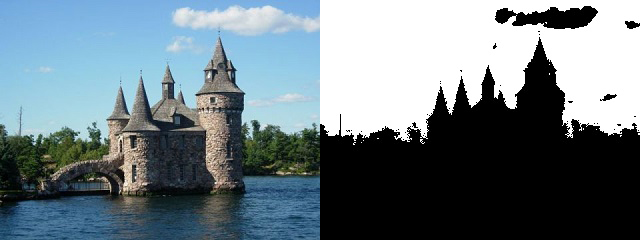
\includegraphics{D:/Workplace/opencv_learn/OpenCV3Cookbook-cn/CH3-image1.jpg}
\caption{}
\end{figure}

Here, a white pixel indicates a positive detection of the sought color,
and black indicates negative.

这里,白色像素表示所寻找颜色的正检测,黑色表示负。

Obviously, the algorithm we encapsulated in this class is relatively
simple (as we will see next, it is composed of just one scanning loop
and one tolerance parameter). The Strategy design pattern becomes really
powerful when the algorithm to be implemented is more complex, has many
steps, and includes several parameters.

显然,我们封装在这个类中的算法相对简单(我们将在下面看到,它只由一个扫描循环和一个容差参数组成)。当要实现的算法更复杂,步骤多,并且包含多个参数时,策略设计模式变得非常强大。

\hypertarget{header-n1180}{%
\subsubsection{How it works\ldots{}}\label{header-n1180}}

The core process of this algorithm is easy to build. It is a simple
scanning loop that goes over each pixel,comparing its color with the
target color. Using what we learned in the \emph{Scanning an image with
iterators} recipe of the previous chapter, this loop can be written as
follows:

该算法的核心过程易于构建。这是一个简单的扫描循环,遍历每个像素,将其颜色与目标颜色进行比较。使用我们在上一章的使用迭代器配方扫描图像中学到的知识,可以按如下方式编写此循环:

\begin{Shaded}
\begin{Highlighting}[]
\CommentTok{// get the iterators}
\NormalTok{cv::Mat_<cv::Vec3b>::const_iterator it= image.begin<cv::Vec3b>();}
\NormalTok{cv::Mat_<cv::Vec3b>::const_iterator itend= image.end<cv::Vec3b>();}
\NormalTok{cv::Mat_<}\ExtensionTok{uchar}\NormalTok{>::iterator itout= result.begin<}\ExtensionTok{uchar}\NormalTok{>();}
\CommentTok{//for each pixel}
\ControlFlowTok{for}\NormalTok{ ( ; it!= itend; ++it, ++itout) \{}
    \CommentTok{// compute distance from target color}
    \ControlFlowTok{if}\NormalTok{ (getDistanceToTargetColor(*it)<=maxDist) \{}
\NormalTok{    	*itout= }\DecValTok{255}\NormalTok{;}
\NormalTok{    \} }\ControlFlowTok{else}\NormalTok{ \{}
\NormalTok{    	*itout= }\DecValTok{0}\NormalTok{;}
\NormalTok{    \}}
\NormalTok{\}}
\end{Highlighting}
\end{Shaded}

The \texttt{cv::Mat} variable \texttt{image} refers to the input image,
while \texttt{result} refers to the binary output image.Therefore, the
first step consists of setting up the required iterators. The scanning
loop then becomes easy to implement. Note that the input image iterators
are declared \texttt{const} as the values of their elements are not
modified. The distance between the current pixel color and the target
color is evaluated for each pixel in order to check whether it is within
the tolerance parameter defined by \texttt{maxDist}. If that is the
case, the value \texttt{255} (white) is then assigned to the output
image; if not, 0 (black) is assigned. To compute the distance to the
target color, the \texttt{getDistanceToTargetColor} method is used.
There are different ways to compute this distance.

\texttt{cv::Mat}变量\texttt{image}是指输入图像,而\texttt{result}是指二进制输出图像。因此,第一步是设置所需的迭代器。然后扫描循环变得易于实现。请注意,输入图像迭代器被声明为``const'',因为它们的元素值不会被修改。针对每个像素评估当前像素颜色和目标颜色之间的距离,以检查它是否在由``maxDist''定义的容差参数内。如果是这种情况,则将值``255''(白色)分配给输出图像;如果不是,则分配0(黑色)。要计算到目标颜色的距离,使用\texttt{getDistanceToTargetColor}方法。有不同的方法来计算这个距离。

One could, for example, calculate the Euclidean distance between the
three vectors that contain the RGB color values. To keep this
computation simple, we sum the absolute differences of the RGB values
(this is also known as the \textbf{city-block distance}). Note that in
modern architecture, a floating-point Euclidean distance can be faster
to compute than a simple city-block distance (in addition, you can also
use squared Euclidean distances to avoid the costly square-root); this
is also something to take into consideration in your design.Also, for
more flexibility, we write the \texttt{getDistanceToTargetColor} method
in terms of a getColorDistance method, as follows:

例如,可以计算包含RGB颜色值的三个矢量之间的欧几里德距离。为了简化这个计算,我们总结了RGB值的绝对差值(这也称为\textbf{city-block
distance})。请注意,在现代建筑中,浮点欧几里德距离的计算速度可能比简单的城块距离更快(此外,您还可以使用平方欧几里德距离来避免昂贵的平方根);这也是你的设计中需要考虑的因素。另外,为了更加灵活,我们根据\texttt{getColorDistance}方法编写\texttt{getDistanceToTargetColor}方法,如下所示:

\begin{Shaded}
\begin{Highlighting}[]
\CommentTok{// Computes the distance from target color.}
\DataTypeTok{int}\NormalTok{ getDistanceToTargetColor(}\AttributeTok{const}\NormalTok{ cv::Vec3b& color) }\AttributeTok{const}\NormalTok{ \{}
	\ControlFlowTok{return}\NormalTok{ getColorDistance(color, target);}
\NormalTok{\}}
\CommentTok{// Computes the city-block distance between two colors.}
\DataTypeTok{int}\NormalTok{ getColorDistance(}\AttributeTok{const}\NormalTok{ cv::Vec3b& color1,}
\AttributeTok{const}\NormalTok{ cv::Vec3b& color2) }\AttributeTok{const}\NormalTok{ \{}
    \ControlFlowTok{return}\NormalTok{ abs(color1[}\DecValTok{0}\NormalTok{]-color2[}\DecValTok{0}\NormalTok{])+}
\NormalTok{           abs(color1[}\DecValTok{1}\NormalTok{]-color2[}\DecValTok{1}\NormalTok{])+}
\NormalTok{           abs(color1[}\DecValTok{2}\NormalTok{]-color2[}\DecValTok{2}\NormalTok{]);}
\NormalTok{\}}
\end{Highlighting}
\end{Shaded}

Note how we used \texttt{cv::Vec3d} to hold the three unsigned chars
that represent the RGB values of a color.The \texttt{target} variable
obviously refers to the specified target color, and as we will see, it
is defined as a member variable in the class algorithm that we will
define.Now, let's complete the definition of the processing method.
Users will provide an input image, and the result will be returned once
the image scanning is completed:

注意我们如何使用\texttt{cv::Vec3d}来保存表示颜色的RGB值的三个无符号字符。``target''变量显然是指指定的目标颜色,正如我们将看到的,它被定义为成员我们将定义的类算法中的变量。现在,让我们完成处理方法的定义。用户将提供输入图像,并在图像扫描完成后返回结果:

\begin{Shaded}
\begin{Highlighting}[]
\NormalTok{cv::Mat ColorDetector::process(}\AttributeTok{const}\NormalTok{ cv::Mat &image) \{}
    \CommentTok{// re-allocate binary map if necessary}
    \CommentTok{// same size as input image, but 1-channel}
\NormalTok{    result.create(image.size(),CV_8U);}
    \CommentTok{// processing loop above goes here}
    \ControlFlowTok{return}\NormalTok{ result;}
\NormalTok{\}}
\end{Highlighting}
\end{Shaded}

Each time this method is called, it is important to check if the output
image that contains the resulting binary map needs to be reallocated to
fit the size of the input image. This is why we use the \texttt{create}
method of \texttt{cv::Mat}. Remember that this method will only proceed
to reallocation if the specified size and/or depth do not correspond to
the current image structure.

每次调用此方法时,检查包含生成的二进制映射的输出图像是否需要重新分配以适合输入图像的大小非常重要。这就是我们使用\texttt{cv::Mat}的\texttt{create}方法的原因。请记住,如果指定的大小和/或深度与当前图像结构不对应,则此方法将仅继续重新分配。

Now that we have the core processing method defined, let's see what
additional methods should be added in order to deploy this algorithm. We
have previously determined what input and output data our algorithm
requires. Therefore, we define the class attributes that will hold this
data:

现在我们已经定义了核心处理方法,让我们看看为了部署这个算法应该添加哪些额外的方法。我们之前已经确定了算法所需的输入和输出数据。因此,我们定义将保存此数据的类属性:

\begin{Shaded}
\begin{Highlighting}[]
\KeywordTok{class}\NormalTok{ ColorDetector \{}
    \KeywordTok{private}\NormalTok{:}
    \CommentTok{// minimum acceptable distance}
    \DataTypeTok{int}\NormalTok{ maxDist;}
    \CommentTok{// target color}
\NormalTok{    cv::Vec3b target;}
    \CommentTok{// image containing resulting binary map}
\NormalTok{    cv::Mat result;}
\end{Highlighting}
\end{Shaded}

In order to create an instance of the class that encapsulates our
algorithm (which we have named \texttt{ColorDetector}), we need to
define a constructor. Remember that one of the objectives of the
Strategy design pattern is to make algorithm deployment as easy as
possible. The simplest constructor that can be defined is an empty one.
It will create an instance of the class algorithm in a valid state. We
then want the constructor to initialize all the input parameters to
their default values (or the values that are known to generally give a
good result). In our case, we decided that a distance of 100 is
generally an acceptable tolerance parameter. We also set the default
target color. We chose black for no particular reason. The idea is to
make sure we always start with predictable and valid input values:

为了创建封装我们的算法(我们命名为\texttt{ColorDetector})的类的实例,我们需要定义一个构造函数。请记住,策略设计模式的目标之一是尽可能简化算法部署。可以定义的最简单的构造函数是空的。它将在有效状态下创建类算法的实例。然后,我们希望构造函数将所有输入参数初始化为其默认值(或者已知通常会产生良好结果的值)。在我们的例子中,我们认为距离100通常是可接受的公差参数。我们还设置了默认目标颜色。我们选择黑色没有特别的原因。我们的想法是确保始终以可预测且有效的输入值开头:

\begin{Shaded}
\begin{Highlighting}[]
\CommentTok{// empty constructor}
\CommentTok{// default parameter initialization here}
\NormalTok{ColorDetector() : maxDist(}\DecValTok{100}\NormalTok{), target(}\DecValTok{0}\NormalTok{,}\DecValTok{0}\NormalTok{,}\DecValTok{0}\NormalTok{) \{\}}
\end{Highlighting}
\end{Shaded}

Another option would have been not create an empty constructor and
rather force the user to input a target color and a color distance in a
more elaborated({[}i'læbәreit{]}a. 精细的, 详尽的, 精心计划(或制作)的vt.
详细地说明, 用心地制作, 发挥vi. 变复杂, 作详细说明) constructor:

另一种选择不是创建一个空构造函数,而是强制用户在更精细的构造函数中输入目标颜色和颜色距离:

\begin{Shaded}
\begin{Highlighting}[]
\CommentTok{// another constructor with target and distance}
\NormalTok{ColorDetector(}\ExtensionTok{uchar}\NormalTok{ blue, }\ExtensionTok{uchar}\NormalTok{ green, }\ExtensionTok{uchar}\NormalTok{ red, }\DataTypeTok{int}\NormalTok{ mxDist);}
\end{Highlighting}
\end{Shaded}

At this point, a user who creates an instance of our class algorithm can
immediately call the process method with a valid image and obtain a
valid output. This is another objective of the Strategy pattern, that
is, to make sure that the algorithm always runs with valid parameters.
Obviously, the users of this class will want to use their own settings.
This is done by providing the user with the appropriate getters and
setters. Let's start with the color tolerance parameter:

此时,创建类算法实例的用户可以立即使用有效图像调用process方法并获取有效输出。这是策略模式的另一个目标,即确保算法始终使用有效参数运行。显然,这个类的用户会想要使用自己的设置。这是通过向用户提供适当的getter和setter来完成的。让我们从颜色容差参数开始:

\begin{Shaded}
\begin{Highlighting}[]
\CommentTok{// Sets the color distance threshold}
\CommentTok{// Threshold must be positive,}
\CommentTok{// otherwise distance threshold is set to 0.}
\DataTypeTok{void}\NormalTok{ setColorDistanceThreshold(}\DataTypeTok{int}\NormalTok{ distance) \{}
    \ControlFlowTok{if}\NormalTok{ (distance<}\DecValTok{0}\NormalTok{)}
\NormalTok{    	distance=}\DecValTok{0}\NormalTok{;}
\NormalTok{    maxDist= distance;}
\NormalTok{\}}
\CommentTok{// Gets the color distance threshold}
\DataTypeTok{int}\NormalTok{ getColorDistanceThreshold() }\AttributeTok{const}\NormalTok{ \{}
	\ControlFlowTok{return}\NormalTok{ maxDist;}
\NormalTok{\}}
\end{Highlighting}
\end{Shaded}

Note how we first check the validity( {[}va·lid·i·ty
\textbar{}\textbar{} və'lɪdətɪ{]}n. 有效性; 正确性; 合法性) of the
input. Again, this is to make sure that our algorithm will never be run
in an invalid state. The target color can be set in a similar manner, as
follows:

请注意我们如何首先检查输入的有效性。同样,这是为了确保我们的算法永远不会在无效状态下运行。可以以类似的方式设置目标颜色,如下所示:

\begin{Shaded}
\begin{Highlighting}[]
\CommentTok{// Sets the color to be detected}
\DataTypeTok{void}\NormalTok{ setTargetColor(}\ExtensionTok{uchar}\NormalTok{ blue, }\ExtensionTok{uchar}\NormalTok{ green, }\ExtensionTok{uchar}\NormalTok{ red) \{}
    \CommentTok{// BGR order}
\NormalTok{    target = cv::Vec3b(blue, green, red);}
\NormalTok{\}}
\CommentTok{// Sets the color to be detected}
\DataTypeTok{void}\NormalTok{ setTargetColor(cv::Vec3b color) \{}
\NormalTok{    target= color;}
\NormalTok{\}}
\CommentTok{// Gets the color to be detected}
\NormalTok{cv::Vec3b getTargetColor() }\AttributeTok{const}\NormalTok{ \{}
    \ControlFlowTok{return}\NormalTok{ target;}
\NormalTok{\}}
\end{Highlighting}
\end{Shaded}

This time, it is interesting to note that we have provided the user with
two definitions of the \texttt{setTargetColor} method. In the first
version of the definition, the three color components are specified as
three arguments, while in the second version, \texttt{cv::Vec3b} is used
to hold the color values. Again, the objective is to facilitate the use
of our class algorithm. The users can simply select the setter that best
fits their needs.

这一次,有趣的是我们已经为用户提供了\texttt{setTargetColor}方法的两个定义。在定义的第一个版本中,三个颜色组件被指定为三个参数,而在第二个版本中,\texttt{cv::Vec3b}用于保存颜色值。同样,目标是促进我们的类算法的使用。用户可以简单地选择最适合他们需求的setter。

\hypertarget{header-n1211}{%
\subsubsection{There's more\ldots{}}\label{header-n1211}}

The example algorithm used in this recipe consisted of identifying the
pixels of an image that has a color sufficiently close to a specified
target color. This computation could have been done
otherwise.Interestingly, an OpenCV function performs a similar task in
order to extract a connected component of a given color. Also, the
implementation of a Strategy design pattern could be complemented using
function objects. Finally, OpenCV has defined a base class,
\texttt{cv::Algorithm}, that implements the Strategy design pattern
concepts.

这节中使用的示例算法包括识别具有足够接近指定目标颜色的颜色的图像的像素。这种计算可能已经完成。有趣的是,OpenCV函数执行类似的任务以便提取给定颜色的连通分量。此外,可以使用函数对象来补充策略设计模式的实现。最后,OpenCV定义了一个基类\texttt{cv::Algorithm},它实现了Strategy设计模式的概念。

\hypertarget{header-n1214}{%
\subsubsection{Computing the distance between two color vectors
}\label{header-n1214}}

To compute the distance between two color vectors, we used the following
simple formula:

为了计算两个颜色向量之间的距离,我们使用了以下简单公式:

\begin{Shaded}
\begin{Highlighting}[]
\ControlFlowTok{return}\NormalTok{ abs(color[}\DecValTok{0}\NormalTok{]-target[}\DecValTok{0}\NormalTok{])+abs(color[}\DecValTok{1}\NormalTok{]-target[}\DecValTok{1}\NormalTok{])+abs(color[}\DecValTok{2}\NormalTok{]-target[}\DecValTok{2}\NormalTok{]);}
\end{Highlighting}
\end{Shaded}

However, OpenCV includes a function to compute the Euclidean norm of a
vector.Consequently, we could have computed our distance as follows:

然而,OpenCV包含一个计算向量的欧几里德范数的函数。因此,我们可以计算我们的距离如下:

\begin{Shaded}
\begin{Highlighting}[]
\ControlFlowTok{return} \KeywordTok{static_cast}\NormalTok{<}\DataTypeTok{int}\NormalTok{>(cv::norm<}\DataTypeTok{int}\NormalTok{,}\DecValTok{3}\NormalTok{>(cv::Vec3i(color[}\DecValTok{0}\NormalTok{]-target[}\DecValTok{0}\NormalTok{],color[}\DecValTok{1}\NormalTok{]-target[}\DecValTok{1}\NormalTok{],color[}\DecValTok{2}\NormalTok{]-target[}\DecValTok{2}\NormalTok{])));}
\end{Highlighting}
\end{Shaded}

A very similar result would then be obtained using this definition of
the getDistance method. Here, we use cv::Vec3i (a 3-vector array of
integers) because the result of the subtraction is an integer value.

然后使用getDistance方法的这个定义获得非常相似的结果。这里,我们使用cv ::
Vec3i(一个3向量的整数数组),因为减法的结果是一个整数值。

It is also interesting to recall from Chapter 2, Manipulating Pixels,
that the OpenCV matrix and vector data structures include a definition
of the basic arithmetic operators.Consequently, one could have proposed
the following definition for the distance computation:

从第2章,操纵像素回忆起,OpenCV矩阵和矢量数据结构包括基本算术运算符的定义也是有趣的。因此,可以为距离计算提出以下定义:

\begin{Shaded}
\begin{Highlighting}[]
\ControlFlowTok{return} \KeywordTok{static_cast}\NormalTok{<}\DataTypeTok{int}\NormalTok{>( cv::norm<}\ExtensionTok{uchar}\NormalTok{,}\DecValTok{3}\NormalTok{>(color-target));}\CommentTok{// wrong!}
\end{Highlighting}
\end{Shaded}

This definition may look right at the first glance; however, it is
wrong. This is because all these operators always include a call to
saturate\_cast (see the Scanning an image with neighbor access recipe in
the previous chapter) in order to ensure that the results stay within
the domain of the input type (here, it is uchar). Therefore, in the
cases where the target value is greater than the corresponding color
value, the value 0 will be assigned instead of the negative value that
one would have expected. A correct formulation would then be as follows:

乍一看,这个定义可能看起来正确;但是,这是错误的。这是因为所有这些运算符总是包含对saturate\_cast的调用(请参阅上一章中使用邻居访问扫描图像的内容),以确保结果保持在输入类型的域内(此处为uchar)。因此,在目标值大于相应颜色值的情况下,将分配值0而不是人们预期的负值。那么正确的表述如下:

\begin{Shaded}
\begin{Highlighting}[]
\NormalTok{cv::Vec3b dist;}
\NormalTok{cv::absdiff(color,target,dist);}
\ControlFlowTok{return}\NormalTok{ cv::sum(dist)[}\DecValTok{0}\NormalTok{];}
\end{Highlighting}
\end{Shaded}

However, using two function calls to compute the distance between two
3-vector arrays is inefficient.

但是,使用两个函数调用来计算两个3向量数组之间的距离是低效的。

\hypertarget{header-n1231}{%
\subsubsection{Using OpenCV functions }\label{header-n1231}}

In this recipe, we used a loop with iterators in order to perform our
computation.Alternatively, we could have achieved the same result by
calling a sequence of OpenCV functions. The color detection method will
then be written as follows:

在本节中,我们使用了一个带迭代器的循环来执行我们的计算。或者,我们可以通过调用一系列OpenCV函数来实现相同的结果。然后将颜色检测方法写成如下:

\begin{Shaded}
\begin{Highlighting}[]
\NormalTok{cv::Mat ColorDetector::process(}\AttributeTok{const}\NormalTok{ cv::Mat &image) \{}
\NormalTok{    cv::Mat output;}
    \CommentTok{// compute absolute difference with target color}
\NormalTok{    cv::absdiff(image,cv::Scalar(target),output);}
    \CommentTok{// split the channels into 3 images}
    \BuiltInTok{std::}\NormalTok{vector<cv::Mat> images;}
\NormalTok{    cv::split(output,images);}
    \CommentTok{// add the 3 channels (saturation might occurs here)}
\NormalTok{    output= images[}\DecValTok{0}\NormalTok{]+images[}\DecValTok{1}\NormalTok{]+images[}\DecValTok{2}\NormalTok{];}
    \CommentTok{// apply threshold}
\NormalTok{    cv::threshold(output, }\CommentTok{// same input/output image}
\NormalTok{                  output,}
\NormalTok{                  maxDist, }\CommentTok{// threshold (must be < 256)}
                  \DecValTok{255}\NormalTok{, }\CommentTok{// max value}
\NormalTok{                  cv::THRESH_BINARY_INV); }\CommentTok{// thresholding mode}
    \ControlFlowTok{return}\NormalTok{ output;}
\NormalTok{\}}
\end{Highlighting}
\end{Shaded}

This method uses the \texttt{absdiff} function, which computes the
absolute difference between the pixels of an image and, in this case, a
scalar value. Instead of a scalar value, another image can be provided
as the second argument to this function. In the latter case, a
pixel-bypixel difference will be applied; consequently, the two images
must be of the same size. The individual channels of the difference
image are then extracted using the \texttt{split} function (discussed in
the \href{}{There's more\ldots{}} section of the
\emph{\href{}{Performing simple image arithmetic}} recipe of
\href{}{Chapter 2, Manipulating Pixels}) in order to be able to add them
together. It is important to note that the result of this sum may
sometimes be greater than 255, but because saturation is always applied,
the result will be stopped at 255. The consequence is that with this
version, the \texttt{maxDist} parameter must also be less than 256; this
should be corrected if you consider this behavior unacceptable.

此方法使用\texttt{absdiff}函数,该函数计算图像像素之间的绝对差值,在本例中为标量值。可以提供另一个图像作为此函数的第二个参数,而不是标量值。在后一种情况下,将应用逐像素差异;因此,两个图像必须具有相同的大小。然后使用\texttt{split}函数提取差分图像的各个通道(在\href{}{第2章,操作像素}的
\href{}{\emph{执行简单图像算术}}配方的\href{}{There's
more\ldots{}}部分中讨论过)以便能够将它们加在一起。重要的是要注意,此总和的结果有时可能大于255,但由于总是应用饱和,结果将在255处停止。结果是,对于此版本,\texttt{maxDist}参数也必须小于超过256;如果您认为此行为不可接受,则应予以纠正。

The last step is to create a binary image by using the
\texttt{cv::threshold} function. This function is commonly used to
compare all the pixels with a threshold value (the third parameter), and
in the regular thresholding mode (\texttt{cv::THRESH\_BINARY}), it
assigns the defined maximum value (the fourth parameter) to all the
pixels greater than the specified threshold and 0 to the other pixels.
Here, we used the inverse mode (\texttt{cv::THRESH\_BINARY\_INV}) in
which the defined maximum value is assigned to the pixels that have a
value lower than or equal to the threshold. Of interest are also the
\texttt{cv::THRESH\_TOZERO} and \texttt{cv::THRESH\_TOZERO\_INV} modes,
which leave the pixels greater than or lower than the threshold
unchanged.

最后一步是使用\texttt{cv::threshold}函数创建二进制映像。此函数通常用于将所有像素与阈值(第三个参数)进行比较,在常规阈值模式(\texttt{cv::THRESH\_BINARY})中,它将定义的最大值(第四个参数)分配给所有像素大于指定的阈值,0到其他像素。这里,我们使用逆模式(\texttt{cv::THRESH\_BINARY\_INV}),其中定义的最大值被分配给值小于或等于阈值的像素。有趣的是\texttt{cv::THRESH\_TOZERO}和\texttt{cv::THRESH\_TOZERO\_INV}模式,它们使像素大于或低于阈值时保持不变。

Using the OpenCV functions is generally a good idea. You can then
quickly build complex applications and potentially reduce the number of
bugs. The result is often more efficient (thanks to the optimization
efforts invested by the OpenCV contributors). However, when many
intermediate steps are performed, you may find that the resulting method
consumes more memory.

使用OpenCV函数通常是个好主意。然后,您可以快速构建复杂的应用程序,并可能减少错误的数量。结果通常更有效(归功于OpenCV贡献者投入的优化努力)。但是,当执行许多中间步骤时,您可能会发现生成的方法会占用更多内存。

\hypertarget{header-n1241}{%
\subsubsection{The floodFill function}\label{header-n1241}}

Our \texttt{ColorDetector} class identifies the pixels in an image that
have a color similar to a given target color. The decision to accept or
not a pixel is simply made on a per-pixel basis.The
\texttt{cv::floodFill} function proceeds in a very similar way with one
important difference: in this case, the decision to accept a pixel also
depends on the state of its neighbors. The idea is to identify a
connected area of a certain color. The user specifies a starting pixel
location and tolerance parameters that determine color similarity.

我们的\texttt{ColorDetector}类识别图像中颜色与给定目标颜色相似的像素。接受或不接受像素的决定只是基于每个像素进行.\texttt{cv\ ::\ floodFill}函数以非常类似的方式进行,但有一个重要区别:在这种情况下,接受像素的决定也依赖于相邻像素的状况。想法是识别某种颜色的连接区域。用户指定确定颜色相似性的起始像素位置和公差参数。

The seed pixel defines the color that is seek and from this seed
location, the neighbors are considered in order to identify pixels of
similar color; then the neighbors of the accepted neighbors are also
considered and so on. This way, one area of constant color will be
extracted from the image. For example, to detect the blue sky area in
our example image,you could proceed as follows:

种子像素定义寻找的颜色,并且从该种子位置,考虑相邻相熟以识别相似颜色的像素;然后也考虑接受的邻居的邻居等等。这样,将从图像中提取一个恒定颜色的区域。例如,要检测示例图像中的蓝天区域,可以按以下步骤操作:

\begin{Shaded}
\begin{Highlighting}[]
\NormalTok{cv::floodFill(image, }\CommentTok{// input/ouput image}
\NormalTok{              cv::Point(}\DecValTok{100}\NormalTok{, }\DecValTok{50}\NormalTok{), }\CommentTok{// seed point}
\NormalTok{              cv::Scalar(}\DecValTok{255}\NormalTok{, }\DecValTok{255}\NormalTok{, }\DecValTok{255}\NormalTok{), }\CommentTok{// repainted color}
\NormalTok{              (cv::Rect*)}\DecValTok{0}\NormalTok{, }\CommentTok{// bounding rect of the repainted set}
\NormalTok{              cv::Scalar(}\DecValTok{35}\NormalTok{, }\DecValTok{35}\NormalTok{, }\DecValTok{35}\NormalTok{), }\CommentTok{// low/high difference threshold}
\NormalTok{              cv::Scalar(}\DecValTok{35}\NormalTok{, }\DecValTok{35}\NormalTok{, }\DecValTok{35}\NormalTok{), }\CommentTok{// identical most of the time}
\NormalTok{              cv::FLOODFILL_FIXED_RANGE);}\CommentTok{// pixels compared to seed}
\end{Highlighting}
\end{Shaded}

The seed pixel (100, 50) is located in the sky. All connected pixels
will be tested and the ones having a similar color will be repainted in
a new color specified by the third parameter. To determine if a color is
similar or not, different thresholds are defined independently for
values that are higher or lower than the reference color. Here, we used
fixed range mode, which implies that the tested pixels will all be
compared to the seed pixel's color. The default mode is the one where
each tested pixel is compared to the color of its neighbors. The result
obtained is as follows:

种子像素(100,50)位于天空中。将测试所有连接的像素,并且将以由第三参数指定的新颜色重新绘制具有相似颜色的像素。为了确定颜色是否相似,对于高于或低于参考颜色的值,独立地定义不同的阈值。在这里,我们使用固定范围模式,这意味着测试的像素将全部与种子像素的颜色进行比较。默认模式是将每个测试像素与其邻居的颜色进行比较的模式。获得的结果如下:(左边是原始图像,右边是处理过后的图像)

\begin{figure}
\centering
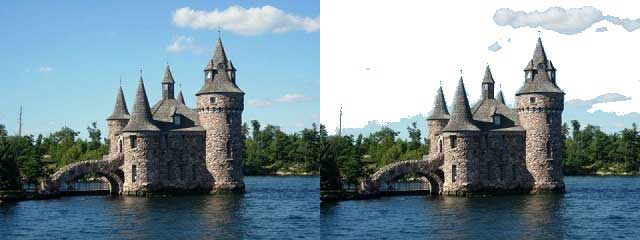
\includegraphics{D:/Workplace/opencv_learn/OpenCV3Cookbook-cn/CH3-image2.jpg}
\caption{}
\end{figure}

A single connected area is repainted by the algorithm (here, we painted
the sky in white).Therefore, even if there are some pixels somewhere
else with a similar color (in the water,for instance), these ones would
not be identified unless they were connected to the sky area.

算法重新绘制了一个连接的区域(这里,我们将天空涂成白色)。因此,即使其他地方有一些具有相似颜色的像素(例如在水中),这些也不会被识别出来。他们连接到天空区域。

\hypertarget{header-n1252}{%
\subsubsection{Functor or function object}\label{header-n1252}}

Using the C++ operator overloading, it is possible to create a class for
which its instances behave as functions. The idea is to overload the
\texttt{operator()} method so that a call to the processing method of a
class looks exactly like a simple function call. The resulting class
instance is called a function object, or a \texttt{functor}.Often, a
functor includes a full constructor such that it can be used immediately
after being created.For example, you can define the full constructor of
your ColorDetector class as follows:

使用C
++运算符重载,可以创建一个类,其实例表现为函数。我们的想法是重载\texttt{operator()}方法,以便对类的处理方法的调用看起来就像一个简单的函数调用。生成的类实例称为函数对象或函数。通常情况下,仿函数包含一个完整的构造函数,以便在创建后立即使用它。例如,您可以按如下方式定义ColorDetector类的完整构造函数:

\begin{Shaded}
\begin{Highlighting}[]
\CommentTok{// full constructor}
\NormalTok{ColorDetector(}\ExtensionTok{uchar}\NormalTok{ blue, }\ExtensionTok{uchar}\NormalTok{ green, }\ExtensionTok{uchar}\NormalTok{ red, }\DataTypeTok{int}\NormalTok{ maxDist=}\DecValTok{100}\NormalTok{)}
\NormalTok{    : maxDist(maxDist) \{}
	\CommentTok{// target color}
\NormalTok{	setTargetColor(blue, green, red);}
\NormalTok{\}}
\end{Highlighting}
\end{Shaded}

Obviously, you can still use the setters and getters that have been
defined previously. The functor method can be defined as follows:

显然,您仍然可以使用之前定义的setter和getter方法。仿函数方法可以定义如下:

\begin{Shaded}
\begin{Highlighting}[]
\NormalTok{cv::Mat }\KeywordTok{operator}\NormalTok{()(}\AttributeTok{const}\NormalTok{ cv::Mat &image) \{}
	\CommentTok{// color detection code here}
\NormalTok{\}}
\end{Highlighting}
\end{Shaded}

To detect a given color with this functor method, simply write the
following code snippet:

要使用此仿函数方法检测给定颜色,只需编写以下代码段:

\begin{Shaded}
\begin{Highlighting}[]
\NormalTok{ColorDetector colordetector(}\DecValTok{230}\NormalTok{,}\DecValTok{190}\NormalTok{,}\DecValTok{130}\NormalTok{, }\CommentTok{// color}
\DecValTok{100}\NormalTok{); }\CommentTok{// threshold}
\NormalTok{cv::Mat result= colordetector(image); }\CommentTok{// functor call}
\end{Highlighting}
\end{Shaded}

As you can see, the call to the color detection method now looks like a
function call.

\hypertarget{header-n1263}{%
\subsubsection{The OpenCV base class for algorithms
OpenCV算法基类}\label{header-n1263}}

OpenCV offers many algorithms that perform various computer vision
tasks. To facilitate({[}fә'siliteit{]}vt. 使容易, 促进, 帮助) their use,
most of these algorithms have been made subclass of a generic base class
called \texttt{cv::Algorithm}. This one implements some of the concepts
dictated({[}dɪk'teɪt{]}n:1. an authoritative rule; 2. a guiding
principle. v:1. issue commands or orders for;2. say out loud for the
purpose of recording; 3. rule as a dictator) by the Strategy design
pattern. First, all these algorithms are created dynamically using a
specialized static method that makes sure that the algorithm is always
created in a valid state (that is, with valid default values for the
unspecified parameters). Let's consider, for example, one of these
subclasses, cv::ORB; this one is an interest point operator that will be
discussed in the Detecting FAST features at Multiple Scales recipe in
Chapter 8, Detecting Interest Points. Here,we simply use it as an
illustrative example of an algorithm.

OpenCV提供许多执行各种计算机视觉任务的算法。为了方便它们的使用,这些算法中的大多数已经成为通用基类的子类,称为\texttt{cv::Algorithm}。这个实现了策略设计模式所规定的一些概念。首先,所有这些算法都是使用专门的静态方法动态创建的,该方法确保始终在有效状态下创建算法(即,使用未指定参数的有效默认值)。让我们看下这些子类之一,`cv::ORB子类;这是一个兴趣点操作符,将在第8章``检测兴趣点''中的``多刻度''章节中的``检测FAST''功能中进行讨论。在这里,我们简单地将其用作算法的说明性示例。

An instance of this algorithm is therefore created as follows:

该算法的实例创建如下:

\begin{Shaded}
\begin{Highlighting}[]
\NormalTok{cv::Ptr<cv::ORB> ptrORB = cv::ORB::create(); }\CommentTok{// default state}
\end{Highlighting}
\end{Shaded}

Once created, the algorithm can then be used. For example, the generic
methods \texttt{read} and \texttt{write} can be used to load or store
the state of the algorithm. The algorithms also have specialized methods
(in the case of ORB, for example, the methods \texttt{detect} and
\texttt{compute} can be used to trigger its main computational units).
Algorithms also have specialized setter methods that allows specifying
their internal parameters. Note that we could have declared the pointer
as \texttt{cv::Ptr\textless{}cv::Algorithm\textgreater{}} but, in this
case, we would not be able to use its specialized methods.

一旦创建,就可以使用该算法。例如,通用方法\texttt{read}和\texttt{write}可用于加载或存储算法的状态。算法也有专门的方法(例如,在ORB类中,方法\texttt{detect}和\texttt{compute}可以用来触发它的主要计算单元)。算法也有专门的setter方法,允许指定它们的内部参数。注意我们可以将指针声明为\texttt{cv::Ptr\textless{}cv::Algorithm\textgreater{}},但是,在这种情况下,我们将无法使用其专用方法。

\hypertarget{header-n1271}{%
\subsubsection{See also}\label{header-n1271}}

\begin{itemize}
\item
  The policy-based class design, introduced by A. Alexandrescu, is an
  interesting variant of the Strategy design pattern in which algorithms
  are selected at compile time.由A.
  Alexandrescu引入的基于策略的类设计是策略设计模式的一个有趣变体,其中在编译时选择算法。
\item
  The Converting color representation recipe introduces the concept of
  perceptually uniform color spaces to achieve more intuitive color
  comparison.转换颜色表示配方引入了感知统一颜色空间的概念,以实现更直观的颜色比较。
\end{itemize}

\hypertarget{header-n1277}{%
\subsection{使用GrabCut算法分割图像}\label{header-n1277}}

The previous recipe showed how color information can be useful to
segment an image into area corresponding to specific elements of a
scene. Objects often have distinctive colors, and these ones can often
be extracted by identifying areas of similar colors. OpenCV proposes an
implementation of a popular algorithm for image segmentation: the
\textbf{GrabCut} algorithm. GrabCut is a complex and computationally
expensive algorithm, but it generally produces very accurate results. It
is the best algorithm to use when you want to extract a foreground
object in a still image (for example, to cut and paste an object from
one picture to another)

上一节显示了颜色信息如何用于将图像分割成对应于场景的特定元素的区域。物体通常具有独特的颜色,并且通常可以通过识别相似颜色的区域来提取这些颜色。
OpenCV提出了一种流行的图像分割算法的实现:\textbf{GrabCut}算法。
GrabCut是一种复杂且计算量很大的算法,但它通常会产生非常准确的结果。当您想要在静止图像中提取前景对象时(例如,将对象从一张图片剪切并粘贴到另一张图片中),这是最佳算法。

\hypertarget{header-n1280}{%
\subsubsection{How to do it\ldots{}}\label{header-n1280}}

The \texttt{cv::grabCut} function is easy to use. You just need to input
an image and label some of its pixels as belonging to the background or
to the foreground. Based on this partial labeling, the algorithm will
then determine a foreground/ background segmentation for the complete
image.

\texttt{cv::grabCut}函数很容易使用。您只需输入一个图像并将其某些像素标记为属于背景或前景。基于该部分标记,算法然后将确定完整图像的前景/背景分割。

One way to specify a partial foreground/background labeling for an input
image is by defining a rectangle inside which the foreground object is
included:

为输入图像指定部分前景/背景标注的一种方法是定义一个矩形,其中包含前景对象:

\begin{Shaded}
\begin{Highlighting}[]
\CommentTok{// define bounding rectangle}
\CommentTok{// the pixels outside this rectangle}
\CommentTok{// will be labeled as background}
\NormalTok{cv::Rect rectangle(}\DecValTok{50}\NormalTok{,}\DecValTok{25}\NormalTok{,}\DecValTok{210}\NormalTok{,}\DecValTok{180}\NormalTok{);}
\end{Highlighting}
\end{Shaded}

This defines the following area in the image:

这定义了图像中的以下区域:

\begin{figure}
\centering
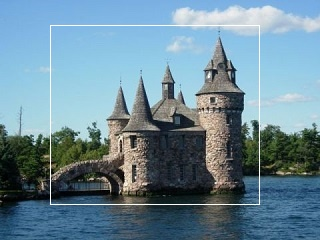
\includegraphics{D:/Workplace/opencv_learn/OpenCV3Cookbook-cn/CH3-image3.jpg}
\caption{}
\end{figure}

All the pixels outside this rectangle will then be marked as background.
In addition to the input image and its segmentation image, calling the
cv::grabCut function requires the definition of two matrices, which will
contain the models built by the algorithm as follows:

此矩形外的所有像素将被标记为背景。除了输入图像及其分割图像之外,调用\texttt{cv::grabCut}函数还需要定义两个矩阵,其中包含算法构建的模型,如下所示:

\begin{Shaded}
\begin{Highlighting}[]
\NormalTok{cv::Mat result; }\CommentTok{// segmentation (4 possible values)}
\NormalTok{cv::Mat bgModel,fgModel; }\CommentTok{// the models (internally used)}
\CommentTok{// GrabCut segmentation}
\NormalTok{cv::grabCut(image, }\CommentTok{// input image}
\NormalTok{            result, }\CommentTok{// segmentation result}
\NormalTok{            rectangle, }\CommentTok{// rectangle containing foreground}
\NormalTok{            bgModel,fgModel, }\CommentTok{// models}
            \DecValTok{5}\NormalTok{, }\CommentTok{// number of iterations}
\NormalTok{            cv::GC_INIT_WITH_RECT); }\CommentTok{// use rectangle}
\end{Highlighting}
\end{Shaded}

Note how we specified that we are using the bounding rectangle mode with
the \texttt{cv::GC\_INIT\_WITH\_RECT} flag as the last argument of the
function (the next section, \emph{How it works\ldots{}}, will discuss
the other available mode). The input/output segmentation image can have
one of the following four values:

注意我们如何指定我们使用带有\texttt{cv::GC\_INIT\_WITH\_RECT}标志的边界矩形模式作为函数的最后一个参数(下一节,\emph{它如何工作......},将讨论其他可用模式)。输入/输出分割图像可以具有以下四个值之一:

\begin{itemize}
\item
  \texttt{cv::GC\_BGD}: This is the value of the pixels that certainly
  belong to the background (for example, pixels outside the rectangle in
  our example)这是当然属于的像素的值背景(例如,我们示例中矩形外的像素)
\item
  \texttt{cv::GC\_FGD}: This is the value of the pixels that certainly
  belong to the foreground (there are none in our
  example)这是当前属于前景的像素值(在我们的示例中没有)
\item
  \texttt{cv::GC\_PR\_BGD}: This is the value of the pixels that
  probably belong to the background这是可能属于背景的像素值
\item
  \texttt{cv::GC\_PR\_FGD}: This is the value of the pixels that
  probably belong to the foreground (that is, the initial value of the
  pixels inside the rectangle in our example)
  这是可能属于前景的像素值(即,我们示例中矩形内的像素的初始值)
\end{itemize}

We get a binary image of the segmentation by extracting the pixels that
have a value equal to \texttt{cv::GC\_PR\_FGD}. This is accomplished
with the following code:

我们通过提取值等于\texttt{cv::GC\_PR\_FGD}的像素来获得分割的二进制图像。这是通过以下代码完成的:

\begin{Shaded}
\begin{Highlighting}[]
\CommentTok{// Get the pixels marked as likely foreground}
\NormalTok{cv::compare(result,cv::GC_PR_FGD,result,cv::CMP_EQ);}
\CommentTok{// Generate output image}
\NormalTok{cv::Mat foreground(image.size(),CV_8UC3,cv::Scalar(}\DecValTok{255}\NormalTok{,}\DecValTok{255}\NormalTok{,}\DecValTok{255}\NormalTok{));}
\NormalTok{image.copyTo(foreground,}\CommentTok{// bg pixels are not copied result);}
\end{Highlighting}
\end{Shaded}

To extract all the foreground pixels, that is, with values equal to
\texttt{cv::GC\_PR\_FGD} or \texttt{cv::GC\_FGD}, it is possible to
check the value of the first bit, as follows:

要提取所有前景像素,即使用等于\texttt{cv::GC\_PR\_FGD}或\texttt{cv::GC\_FGD}的值,可以检查第一位的值,如下所示:

\begin{Shaded}
\begin{Highlighting}[]
\CommentTok{// checking first bit with bitwise-and}
\NormalTok{result= result&}\DecValTok{1}\NormalTok{; }\CommentTok{// will be 1 if FG}
\end{Highlighting}
\end{Shaded}

This is possible because these constants are defined as values 1 and 3,
while the other two (\texttt{cv::GC\_BGD} and \texttt{cv::GC\_PR\_BGD})
are defined as 0 and 2. In our example, the same result is obtained
because the segmentation image does not contain the \texttt{cv::GC\_FGD}
pixels (only the \texttt{cv::GC\_BGD} pixels have been inputted).

这是可能的,因为这些常量定义为值1和3,而另外两个(\texttt{cv::GC\_BGD}和\texttt{cv::GC\_PR\_BGD})定义为0和2.在我们的示例中,获得相同的结果,因为分割图像不包含\texttt{cv::GC\_FGD}像素(仅输入了\texttt{cv::GC\_BGD}像素)。

The following image is then obtained:

\begin{figure}
\centering
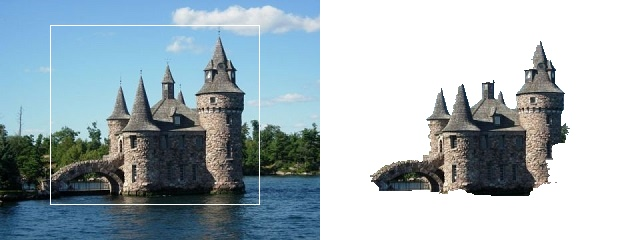
\includegraphics{D:/Workplace/opencv_learn/OpenCV3Cookbook-cn/CH3-image4.jpg}
\caption{}
\end{figure}

\hypertarget{header-n1313}{%
\subsubsection{How it works\ldots{}}\label{header-n1313}}

In the preceding example, the GrabCut algorithm was able to extract the
foreground object by simply specifying a rectangle inside which this
objects (the castle) was contained. Alternatively, one could also assign
the values \texttt{cv::GC\_BGD} and \texttt{cv::GC\_FGD} to some
specific pixels of the input image, which are provided by using a mask
image as the second argument of the \texttt{cv::grabCut} function. You
would then specify \texttt{GC\_INIT\_WITH\_MASK} as the input mode flag.
These input labels could be obtained, for example, by asking a user to
interactively mark a few elements of the image. It is also possible to
combine these two input modes.

在前面的示例中,GrabCut算法能够通过简单地指定包含此对象(城堡)的矩形来提取前景对象。或者,也可以将值\texttt{cv::GC\_BGD}和\texttt{cv::GC\_FGD}分配给输入图像的某些特定像素,这些像素是使用掩码图像作为\texttt{cv::grabCut}的第二个参数提供的。功能。然后,您可以指定\texttt{GC\_INIT\_WITH\_MASK}作为输入模式标志。例如,可以通过要求用户交互地标记图像的一些元素来获得这些输入标签。也可以组合这两种输入模式。

Using this input information, the GrabCut algorithm creates the
background/foreground segmentation by proceeding as follows. Initially,
a foreground label (\texttt{cv::GC\_PR\_FGD}) is
tentatively({[}'ten·ta·tive·ly \textbar{}\textbar{} 'tentətɪvlɪ{]}adv.
试验性地; 暂时地) assigned to all the unmarked pixels. Based on the
current classification, the algorithm groups the pixels into clusters of
similar colors (that is, K clusters for the background and K clusters
for the foreground). The next step is to determine a
background/foreground segmentation by introducing boundaries between the
foreground and background pixels.

使用此输入信息,GrabCut算法通过如下步骤创建背景/前景分割。最初,暂时将前景标签(\texttt{cv::GC\_PR\_FGD})分配给所有未标记的像素。基于当前分类,该算法将像素分组为相似颜色的聚类(即,背景的\(K\)个聚类和前景的\(K\)个聚类)。下一步是通过引入前景像素和背景像素之间的边界来确定背景/前景分割。

This is done through an optimization process that tries to connect
pixels with similar labels, and that imposes({[}im·pose
\textbar{}\textbar{} ɪm'pəʊz{]}v. 征; 把...强加于; 加于; 利用; 施影响;
欺骗) a penalty( {[}'penәlti{]}n. 处罚, 刑罚, 罚款, 罚球, 报应,
不利结果, 妨碍) for placing a boundary in the regions of relatively
uniform intensity. This optimization problem can be efficiently solved
using the Graph Cuts algorithm, a method that can find the optimal
solution of a problem by representing it as a connected graph on which
cuts are applied in order to compose an optimal configuration. The
obtained segmentation produces new labels for the pixels.

这是通过尝试连接具有相似标签的像素的优化过程来完成的,并且这对于在相对均匀强度的区域中放置边界施加了惩罚。使用Graph
Cuts算法可以有效地解决该优化问题,该算法可以通过将其表示为应用了切割的连接图来找到问题的最优解,以便构成最优配置。获得的分割为像素生成新标签。

The clustering process can then be repeated, and a new optimal
segmentation is found again, and so on. Therefore, the GrabCut algorithm
is an iterative procedure that gradually improves the segmentation
result. Depending on the complexity of the scene, a good solution can be
found in more or less number of iterations (in easy cases, one iteration
would be enough).

然后可以重复聚类过程,并再次找到新的最佳分割,等等。
因此,GrabCut算法是一种逐步改进分割结果的迭代过程。
根据场景的复杂程度,可以在或多或少的迭代次数中找到一个好的解决方案(在简单的情况下,一次迭代就足够了)。

This explains the argument of the function where the user can specify
the number of iterations to be applied. The two internal models
maintained by the algorithm are passed as an argument of the function
(and returned). Therefore, it is possible to call the function with the
models of the last run again if one wishes to improve the segmentation
result by performing additional iterations.

这解释了函数的参数,其中用户可以指定要应用的迭代次数。
算法维护的两个内部模型作为函数的参数传递(并返回)。
因此,如果希望通过执行额外的迭代来改进分割结果,则可以再次使用上次运行的模型调用该函数。

\hypertarget{header-n1324}{%
\subsubsection{See also}\label{header-n1324}}

\begin{itemize}
\item
  The article \emph{GrabCut: Interactive Foreground Extraction using
  Iterated Graph Cuts in ACM Transactions on Graphics (SIGGRAPH) volume
  23, issue 3, August 2004, C. Rother, V. Kolmogorov, and A. Blake}
  describes the GrabCut algorithm in detail
\item
  The \emph{Segmenting images using watersheds} recipe in
  \textbf{Chapter 5, Transforming Images with Morphological Operations},
  presents another image segmentation algorithm 
\end{itemize}

\hypertarget{header-n1330}{%
\subsection{转换颜色表示}\label{header-n1330}}

The RGB color space is based on the use of the red, green, and blue
additive primary colors. We saw in the first recipe of this chapter that
these primaries have been chosen because they can produce a good range
of colors well aligned with the human visual system. It is often the
default color space in digital imagery because this is the way color
images are acquired, that is, through the use of red, green, and blue
filters. Additionally, the red, green, and blue channels are normalized
such that when combined in equal amounts, a gray-level intensity is
obtained, that is, from black (0,0,0) to white (255,255,255).

RGB颜色空间基于红色,绿色和蓝色添加剂原色的使用。
我们在本章的第一个章节中看到,选择这些原色是因为它们可以产生与人类视觉系统完全一致的各种颜色。
它通常是数字图像中的默认颜色空间,因为这是获取彩色图像的方式,即通过使用红色,绿色和蓝色滤镜。
另外,红色,绿色和蓝色通道被归一化,使得当以相等的量组合时,获得灰度级强度,即,从黑色(0,0,0)到白色(255,255,255)。

Unfortunately, computing the distance between the colors using the RGB
color space is not the best way to measure the similarity between two
given colors. Indeed, RGB is not a perceptually uniform color space.
This means that two colors at a given distance might look very similar,
while two other colors separated by the same distance might look very
different.

不幸的是,使用RGB颜色空间计算颜色之间的距离并不是测量两种给定颜色之间相似性的最佳方法。
实际上,RGB不是感知上均匀的色彩空间。
这意味着给定距离处的两种颜色可能看起来非常相似,而以相同距离分隔的另外两种颜色可能看起来非常不同。

To solve this problem, other color representations that have the
property of being perceptually uniform have been introduced. In
particular, the \(\text{CIE} \space L^{*}a^{*}b^{*}\) is one such color
model. By converting our images to this representation, the Euclidean
distance between an image pixel and the target color will then be a
meaningful measure of the visual similarity between the two colors. In
this recipe, we will show you how to convert colors from one
representation to another in order to work with other color spaces.

为了解决这个问题,已经引入了具有感知统一特性的其他颜色表示。
特别是,\(\text{CIE} \space L^{*}a^{*}b^{*}\)就是这样一种颜色模型。
通过将我们的图像转换为该表示,图像像素和目标颜色之间的欧几里德距离将是两种颜色之间的视觉相似性的有意义的度量。
在本文中,我们将向您展示如何将颜色从一种表示转换为另一种表示,以便与其他颜色空间一起使用。

\hypertarget{header-n1337}{%
\subsubsection{How to do it\ldots{} }\label{header-n1337}}

Conversion of images between different color spaces is easily done
through the use of the \texttt{cv::cvtColor} OpenCV function. Let's
revisit the \texttt{ColorDetector} class of the first recipe of this
chapter,
\texttt{Comparing\ colors\ using\ the\ Strategy\ design\ pattern}. We
now convert the input image to the \(\text{CIE} \space L^{*}a^{*}b^{*}\)
color space at the beginning of the process method:

通过使用\texttt{cv::cvtColor}
OpenCV函数可以轻松地在不同颜色空间之间转换图像。
让我们重温一下本章第一篇文章的\texttt{ColorDetector}类,\texttt{使用策略设计模式比较颜色}。
我们现在将输入图像转换为处理方法开头的\( \text{CIE} \space L^{*} a^{*} b^{*} \)颜色空间:

\begin{Shaded}
\begin{Highlighting}[]
\NormalTok{cv::Mat ColorDetector::process(}\AttributeTok{const}\NormalTok{ cv::Mat &image) \{}
    \CommentTok{// re-allocate binary map if necessary}
    \CommentTok{// same size as input image, but 1-channel}
\NormalTok{    result.create(image.rows,image.cols,CV_8U);}
    \CommentTok{// Converting to Lab color space}
\NormalTok{    cv::cvtColor(image, converted, CV_BGR2Lab);}
    \CommentTok{// get the iterators of the converted image}
\NormalTok{    cv::Mat_<cv::Vec3b>::iterator it= converted.begin<cv::Vec3b>();}
\NormalTok{    cv::Mat_<cv::Vec3b>::iterator itend= converted.end<cv::Vec3b>();}
    \CommentTok{// get the iterator of the output image}
\NormalTok{    cv::Mat_<}\ExtensionTok{uchar}\NormalTok{>::iterator itout= result.begin<}\ExtensionTok{uchar}\NormalTok{>();}
    \CommentTok{// for each pixel}
    \ControlFlowTok{for}\NormalTok{ ( ; it!= itend; ++it, ++itout) \{}
\end{Highlighting}
\end{Shaded}

The converted variable contains the image after color conversion. In the
ColorDetector class, it is defined as a class attribute:

变量\texttt{converted}包含颜色转换后的图像。
在ColorDetector类中,它被定义为类属性:

\begin{Shaded}
\begin{Highlighting}[]
\KeywordTok{class}\NormalTok{ ColorDetector \{}
\KeywordTok{private}\NormalTok{:}
    \CommentTok{// image containing color converted image}
\NormalTok{    cv::Mat converted;}
\end{Highlighting}
\end{Shaded}

You also need to convert the input target color. You can do this by
creating a temporary image that contains only one pixel. Note that you
need to keep the same signature as in the earlier recipes, that is, the
user continues to supply the target color in RGB:

您还需要转换输入目标颜色。
您可以通过创建仅包含一个像素的临时图像来完成此操作。
请注意,您需要保留与前面内容中相同的签名,即用户继续以RGB格式提供目标颜色:

\begin{Shaded}
\begin{Highlighting}[]
\CommentTok{// Sets the color to be detected}
\DataTypeTok{void}\NormalTok{ setTargetColor(}\DataTypeTok{unsigned} \DataTypeTok{char}\NormalTok{ red, }\DataTypeTok{unsigned} \DataTypeTok{char}\NormalTok{ green, }\DataTypeTok{unsigned} \DataTypeTok{char}\NormalTok{ blue) \{}
    \CommentTok{// Temporary 1-pixel image}
\NormalTok{    cv::Mat tmp(}\DecValTok{1}\NormalTok{,}\DecValTok{1}\NormalTok{,CV_8UC3);}
\NormalTok{    tmp.at<cv::Vec3b>(}\DecValTok{0}\NormalTok{,}\DecValTok{0}\NormalTok{)= cv::Vec3b(blue, green, red);}
    \CommentTok{// Converting the target to Lab color space}
\NormalTok{    cv::cvtColor(tmp, tmp, CV_BGR2Lab);}
\NormalTok{    target= tmp.at<cv::Vec3b>(}\DecValTok{0}\NormalTok{,}\DecValTok{0}\NormalTok{);}
\NormalTok{\}}
\end{Highlighting}
\end{Shaded}

If the application of the preceding({[}pre'ced·ing \textbar{}\textbar{}
prɪ'sɪːdɪŋ{]}adj. 在前的, 在先的; 前面的) recipe is compiled with this
modified class, it will now detect the pixels of the target color using
the \( \text{CIE} \space L^{*} a^{*} b^{*} \) color model.

如果使用此修改后的类编译前面章节的应用程序,它现在将使用\( \text{CIE}  \space L^{*} a^{*} b^{*} \)来检测目标颜色的像素的颜色模型。

\hypertarget{header-n1349}{%
\subsubsection{How it works\ldots{}}\label{header-n1349}}

When an image is converted from one color space to another, a linear or
nonlinear transformation is applied on each input pixel to produce the
output pixels. The pixel type of the output image will match the one of
the input image. Even if you work with 8-bit pixels most of the time,
you can also use a color conversion with floating-point images (in which
case, the pixel values are generally assumed to vary between 0 and 1.0)
or with integer images (with pixels generally varying between 0 and
65535). However, the exact domain of the pixel values depends on the
specific color space and destination image type. For example, with the
\( \text{CIE}  \space L^{*} a^{*} b^{*} \) color space, the L channel,
which represents the brightness of each pixel, varies between 0 and 100,
and it is rescaled between 0 and 255 in the case of the 8-bit images.

当图像从一个颜色空间转换为另一个颜色空间时,在每个输入像素上应用线性或非线性变换以产生输出像素。
输出图像的像素类型将与输入图像的像素类型匹配。
即使您在大多数时间使用8位像素,也可以使用浮点图像的颜色转换(在这种情况下,通常假设像素值在0到1.0之间变化)或整数图像(使用
像素通常在0到65535之间变化)。
但是,像素值的确切域取决于特定的颜色空间和目标图像类型。
例如,对于\( \text{CIE}  \space L^{*} a^{*} b^{*} \)颜色空间,表示每个像素的亮度的L通道在0到100之间变化,并且在8位图像的情况下重新调整在0到255之间。

The a and b channels correspond to the
chromaticity({[}ˌkrəuməˈtisiti{]}色度; 染色性) components. These
channels contain information about the color of a pixel, independent of
its brightness. Their values vary between -127 and 127; for 8-bit
images, 128 is added to each value in order to make it fit within the 0
to 255 interval. However, note that the 8-bit color conversion will
introduce rounding({[}round·ing \textbar{}\textbar{} 'raʊndɪŋ{]}n.制圆;
凑整; 舍入) errors that will make the transformation
imperfectly({[}im'pә:fiktli{]}ad. 不完全地, 有缺点地, 不完备地)
reversible({[}re'vers·i·ble \textbar{}\textbar{} rɪ'vɜrsəbl
/-'vɜːsəbl{]}adj. 可反转的; 可掉换的; 可逆的; 可废弃的).

a和b通道对应于色度分量。 这些通道包含有关像素颜色的信息,与其亮度无关。
它们的值在-127到127之间变化;
对于8位图像,将128添加到每个值,以使其适合0到255的间隔。
但是,请注意,8位颜色转换将引入舍入误差,这将使转换不完全可逆。

Most commonly used color spaces are available. It is just a question of
providing the right color space conversion code to the OpenCV function
(for CIE L\emph{a}b*, this code is CV\emph{BGR2Lab). Among these is
YCrCb, which is the color space used in JPEG compression. To convert a
color space from BGR to YCrCb, the code will be CV}BGR2YCrCb. Note that
all the conversions that involve the three regular primary colors, red,
green, and blue, are available in the RGB and BGR order.

最常用的色彩空间是可用的。
这只是向OpenCV函数提供正确的颜色空间转换代码的问题(对于\( \text{CIE}  \space L^{*} a^{*} b^{*} \),此代码为\texttt{CV\_BGR2Lab})。
其中有YCrCb,它是JPEG压缩中使用的色彩空间。
要将颜色空间从BGR转换为YCrCb,代码将为\texttt{CV\_BGR2YCrCb}。
请注意,所有涉及三种常规原色(红色,绿色和蓝色)的转换都以RGB和BGR顺序提供。

The \( \text{CIE}  \space L^{*} u^{*} v^{*} \) color space is another
perceptually uniform color space. You can convert from BGR to
\(\text{CIE}  \space L^{*} u^{*} v^{*} \)by using the
\texttt{CV\_BGR2Luv} code. Both \( L^{*} a^{*} b^{*} \) and
\( L^{*} u^{*} v^{*} \) use the same conversion formula for the
brightness channel but use a different representation for the
chromaticity channels. Also, note that since these two color spaces
distort( {[}dis·tort \textbar{}\textbar{} dɪ'stɔːt{]}v. 弄歪; 歪曲;
扭曲) the RGB color domain in order to make it
perceptually(\textbf{perception} {[}per·cep·tion \textbar{}\textbar{}
pər'sepʃn /pə'-{]}n. 知觉, 领悟力, 感觉) uniform({[}u·ni·form
\textbar{}\textbar{} 'juːnɪfɔrm /-fɔːm{]}n. 制服adj. 统一的, 始终如一的,
一律的), these transformations are nonlinear (therefore, they are costly
to compute).

\( \text{CIE}  \space L^{*} u^{*} v^{*} \)颜色空间是另一个感知上均匀的颜色空间。
您可以使用CV\_BGR2Luv代码从BGR转换为\(\text{CIE}  \space L^{*} u^{*} v^{*} \)。
\( L^{*} a^{*} b^{*} \)和\( L^{*} u^{*} v^{*} \)都使用相同的亮度通道转换公式,但对色度通道使用不同的表示。
另外,请注意,由于这两个颜色空间会扭曲RGB颜色域以使其在感知上均匀,因此这些变换是非线性的(因此,它们的计算成本很高)。

There is also the CIE XYZ color space (with the CV\_BGR2XYZ code). It is
a standard color space used to represent any perceptible color in a
device-independent way. In the computation of the \(L^{*}u^{*}v^{*}\)
and \(L^{*}a^{*}b^{*}\) color spaces, the XYZ color space is used as an
intermediate representation. The transformation between RGB and XYZ is
linear. It is also interesting to note that the Y channel corresponds to
a gray-level version of the image.

还有CIE XYZ颜色空间(CV\_BGR2XYZ代码)。
它是一种标准颜色空间,用于以与设备无关的方式表示任何可感知的颜色。
在\(L^{*}u^{*}v^{*}\)和\(L^{*}a^{*}b^{*}\)颜色空间的计算中,XYZ颜色空间用作中间表示。
RGB和XYZ之间的转换是线性的。 值得注意的是,Y通道对应于图像的灰度版本。

HSV and HLS are interesting color spaces because they
decompose({[}de·com·pose \textbar{}\textbar{} ‚diːkəm'pəʊz{]}v. 分解;
使腐烂; 被分解; 腐烂) the colors into their hue({[}hjuː{]}n. 色调; 颜色;
样子) and saturation({[}sat·u·ra·tion \textbar{}\textbar{}
‚sætʃə'reɪʃn{]}n. 饱和; 浸透; 浸润, 全部充满; 色彩的纯净,
颜色可以和白色混合的程度) components plus the value or
luminance({[}ˈljuːminəns{]}亮度; 发光度) component, which is a more
natural way for humans to describe colors. The next recipe will present
this color space.

HSV和HLS是有趣的色彩空间,因为它们将色彩分解为色调和饱和度分量加上值或亮度分量,这是人类描述色彩的更自然的方式。
下一章将呈现此色彩空间。

You can also convert color images to gray-level intensities. The output
will be a one-channel image:

您还可以将彩色图像转换为灰度级强度。 输出将是单通道图像:

\begin{Shaded}
\begin{Highlighting}[]
\NormalTok{cv::cvtColor(color, gray, CV_BGR2GRAY);}
\end{Highlighting}
\end{Shaded}

It is also possible to do the conversion in the other direction, but the
three channels of the resulting color image will then be identically
filled with the corresponding values in the gray-level image.

也可以在另一个方向上进行转换,但是所得到的彩色图像的三个通道将用灰度图像中的相应值相同地填充。

\hypertarget{header-n1367}{%
\subsubsection{See also}\label{header-n1367}}

\begin{itemize}
\item
  The \href{}{Using the mean shift algorithm to find an object} recipe
  in \protect\hyperlink{ch4}{Chapter 4, Counting the Pixels with
  Histograms}, uses the HSV color space in order to find an object in an
  image.
\item
  Many good references are available on the color space theory. Among
  them, the following is a complete reference: \href{}{The Structure and
  Properties of Color Spaces and the Representation of Color Images,
  E.Dubois, Morgan and Claypool Publishers, 2009}. 
\end{itemize}

\hypertarget{header-n1374}{%
\subsection{用色调,饱和度和亮度表示颜色}\label{header-n1374}}

In this chapter, we played with image colors. We used different color
spaces and tried to identify image areas of uniform color. The RGB color
space was initially considered, and although it is an effective
representation for the capture and display of colors in electronic
imaging systems, this representation is not very intuitive. Indeed, this
is not the way humans think about colors; they most often describe
colors in terms of their tint, brightness, or colorfulness (that is,
whether it is a vivid or pastel color). A color space based on the
concept of hue, saturation, and brightness has then been introduced to
help users to specify the colors using properties that are more
intuitive to them. In this recipe, we will explore the concepts of hue,
saturation, and brightness as a means to describe colors.

在本章中,我们和图像颜色打交道。
我们使用不同的颜色空间并尝试识别均匀颜色的图像区域。
最初考虑RGB颜色空间,尽管它是电子成像系统中颜色的捕获和显示的有效表示,但这种表示不是非常直观。
实际上,这不是人类对颜色的看法;
他们通常根据色彩,亮度或色彩来描述颜色(即,它是生动的还是柔和的颜色)。
然后引入了基于色调,饱和度和亮度概念的色彩空间,以帮助用户使用更直观的属性来指定颜色。
在这个配方中,我们将探索色调,饱和度和亮度的概念作为描述颜色的方法。

\hypertarget{header-n1377}{%
\subsubsection{How to do it\ldots{}}\label{header-n1377}}

The conversion of a BGR image into another color space is done using the
cv::cvtColor function that was explored in the previous recipe. Here, we
will use the CV\_BGR2HSV conversion code:

使用在前一节中探索过的\texttt{cv::cvtColor}函数将BGR图像转换为另一个颜色空间。
在这里,我们将使用 CV\_BGR2HSV转换代码:

\begin{Shaded}
\begin{Highlighting}[]
\CommentTok{// convert into HSV space}
\NormalTok{cv::Mat hsv;}
\NormalTok{cv::cvtColor(image, hsv, CV_BGR2HSV);}
\end{Highlighting}
\end{Shaded}

We can go back to the BGR space using the CV\_HSV2BGR code. We can
visualize each of the HSV components by splitting the converted image
channels into three independent images, as follows:

我们可以使用CV\_HSV2BGR代码返回BGR空间。
我们可以通过将转换后的图像通道分成三个独立的图像来可视化每个HSV组件,如下所示:

\begin{Shaded}
\begin{Highlighting}[]
\CommentTok{// split the 3 channels into 3 images}
\BuiltInTok{std::}\NormalTok{vector<cv::Mat> channels;}
\NormalTok{cv::split(hsv,channels);}
\CommentTok{// channels[0] is the Hue}
\CommentTok{// channels[1] is the Saturation}
\CommentTok{// channels[2] is the Value}
\end{Highlighting}
\end{Shaded}

Note that the third channel is the value of the color, that is, an
approximate({[}əˈprɔksimeit{]}近似; 近似的; 逼近) measure of the
brightness of the color. Since we are working on 8-bit images, OpenCV
rescales the channel values to cover the 0 to 255 range (except for the
hue, which is rescaled between 0 and 0180 as it will be explained in the
next section). This is very convenient as we are able to display these
channels as gray-level images.

请注意,第三个通道是颜色的值,即颜色亮度的近似度量。
由于我们正在处理8位图像,OpenCV会重新调整通道值以覆盖0到255范围(色调除外,它将在0和0180之间重新调整,如下一节中所述)。
这非常方便,因为我们能够将这些通道显示为灰度图像。

城堡图像的Hue通道(左)、Saturation通道(中)和Value通道(右)的图像如下将如下所示:

\begin{figure}
\centering
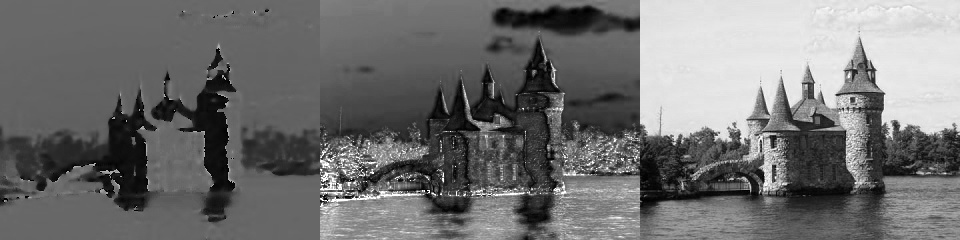
\includegraphics{D:/Workplace/opencv_learn/OpenCV3Cookbook-cn/CH3-image5.jpg}
\caption{}
\end{figure}

\hypertarget{header-n1388}{%
\subsubsection{How it works\ldots{}}\label{header-n1388}}

The hue/saturation/value color space has been introduced because this
representation corresponds to the way humans tend to naturally organize
colors. Indeed, humans prefer to describe colors with intuitive(
{[}in·tu·i·tive \textbar{}\textbar{} ɪn'tuːɪtɪv /-'tju-{]}adj. 直觉的)
attributes such as tint({[}tɪnt{]}n. 色彩, 浅色;v. 给...着色; 使受影响;
染), colorfulness, and brightness. These three attributes are the basis
of most phenomenal( {[}phe·nom·e·nal \textbar{}\textbar{} fɪ'nɑmɪnl
/-'nɒ-{]}adj. 现象的, 异常的, 能知觉的) color spaces. Hue designates(
{[}'dezigneit{]}vt. 指定, 指明, 称呼a. 已选出而未上任的) the dominant
color; the names that we give to colors (such as green, yellow, blue,
and red) correspond to the different hue values. Saturation tells us how
vivid({[}'vivid{]}a. 生动的, 鲜明的, 鲜艳的, 活泼的, 逼真的, 清晰的) the
color is; pastel colors have low saturation, while the colors of the
rainbow are highly saturated. Finally, brightness is a subjective
attribute that refers to the luminosity of a color. Other phenomenal
color spaces use the concept of color value or color lightness as a way
to characterize the relative color intensity.

引入了色调/饱和度/值颜色空间是因为该表示对应于人们自然地组织颜色的倾向。
实际上,人们更喜欢用直观的属性来描述颜色,例如色调,色彩和亮度。
这三个属性是大多数感知色彩空间的基础。 Hue表示主色;
我们给颜色的名称(例如绿色,黄色,蓝色和红色)对应于不同的色调值。
饱和度告诉我们颜色是多么生动;
柔和的颜色具有低饱和度,而彩虹的颜色高度饱和。
最后,亮度是一种主观属性,指的是颜色的亮度。
其他现象色彩空间使用色值或色彩亮度的概念作为表征相对色彩强度的方式。

These color components try to mimic({[}'mimik{]}a. 模仿的, 摹拟的n.
效颦者, 模仿者, 小丑, 仿制品vt. 模仿, 摹拟) the intuitive(
{[}in'tju:itiv{]}a. 直觉的) human perception({[}pә'sepʃәn{]}n. 知觉,
感觉, 领悟力, 获取) of colors. In consequence, there is no standard
definition for them. In the literature, you will find several different
definitions and formulae of the hue, saturation, and brightness. OpenCV
proposes two implementations of phenomenal color spaces: the HSV and the
HLS color spaces. The conversion formulas are slightly different, but
they give very similar results.

这些颜色成分试图模仿人类对颜色的直观感知。 因此,它们没有标准定义。
在文献中,您将找到几种不同的色调,饱和度和亮度的定义和公式。
OpenCV提出了两种现象色彩空间的实现:HSV和HLS色彩空间。
转换公式略有不同,但它们给出了非常相似的结果。

The value component is probably the easiest to interpret. In the OpenCV
implementation of the HSV space, it is defined as the maximum value of
the three BGR components. It is a very simplistic implementation of the
brightness concept. For a definition of brightness that matches the
human visual system better, you should use the L channel of the
perceptually uniform \(L^{*}a^{*}b^{*}\) and \(L^{*}u^{*}v^{*}\) color
spaces. For example, the L channel takes into account the fact that a
green color appears to human brighter than, for instance, a blue color
of same intensity.

值组件可能是最容易解释的。
在HSV空间的OpenCV实现中,它被定义为三个BGR组件的最大值。
这是一个非常简单的亮度概念实现。
对于更好地匹配人类视觉系统的亮度定义,您应该使用感知上均匀的\(L^{*}a^{*}b^{*}\)和
\(L^{*}u^{*}v^{*}\)颜色空间的L通道。
例如,L通道考虑到绿色对人类更亮的事实,例如,相同强度的蓝色。

To compute the saturation, OpenCV uses a formula based on the minimum
and maximum values of the BGR components:

为了计算饱和度,OpenCV使用基于BGR组件的最小值和最大值的公式:

\[\text{S} = \frac{max(R,G,B) - min(R,G,B)}{max(R,G,B)}\]

The idea is that a grayscale color in which the three R, G, and B
components are all equal will correspond to a perfectly desaturated
color; therefore, it will have a saturation value of 0. Saturation is a
value between 0 and 1.0. For 8-bit images, saturation is rescaled to a
value between 0 and 255, and when displayed as a gray-level image,
brighter areas correspond to the colors that have a higher saturation
color.

这个想法是三个R,G和B都相等的灰度颜色将对应于完全去饱和的颜色;
因此,它的饱和度值为0。饱和度是介于0和1.0之间的值。
对于8位图像,饱和度重新调整为0到255之间的值,当显示为灰度图像时,较亮区域对应于具有较高饱和度颜色的颜色。

For example, from the saturation image in the previous section, it can
be seen that the blue of the water is more saturated than the light blue
pastel color of the sky, as expected. The different shades of gray have,
by definition, a saturation value equal to zero (because, in this case,
all three BGR components are equal). This can be observed on the
different roofs of the castle, which are made of a dark gray stone.
Finally, in the saturation image, you may have noticed some white spots
located in areas that correspond to very dark regions of the original
image. These are a consequence of the used definition for saturation.
Indeed, because saturation measures only the relative difference between
the maximum and minimum BGR values, a triplet such as (1,0,0) gives a
perfect saturation of 1.0, even if this color would be seen as black.
Consequently, the saturation values measured in dark regions are
unreliable and should not be considered.

例如,从前一部分的饱和度图像可以看出,水的蓝色比天空的淡蓝色柔和色更饱和,如预期的那样。
根据定义,不同的灰色阴影具有等于零的饱和度值(因为,在这种情况下,所有三个BGR分量都相等)。
这可以在城堡的不同屋顶上观察到,这些屋顶由深灰色的石头制成。
最后,在饱和度图像中,您可能已经注意到位于对应于原始图像的非常暗区域的区域中的一些白点。
这些是使用饱和度定义的结果。
实际上,因为饱和度仅测量最大和最小BGR值之间的相对差异,所以诸如(1,0,0)的三元组给出1.0的完美饱和度,即使该颜色将被视为黑色。
因此,在暗区域中测量的饱和度值是不可靠的,不应该考虑。

The hue of a color is generally represented by an angle value between 0
and 360, with the red color at 0 degrees. In the case of an 8-bit image,
OpenCV divides this angle by two to fit within the 1-byte range.
Therefore, each hue value corresponds to a given color tint independent
of its brightness and saturation. For example, both the sky and the
water have the same hue value, approximately 200 degrees (intensity,
100), which corresponds to the blue shade; the green color of the trees
in the background has a hue of around 90 degrees. It is important to
note that hue is less reliable when evaluated for colors that have a
very low saturation.

颜色的色调通常由0到360之间的角度值表示,红色在0度。
在8位图像的情况下,OpenCV将该角度除以2以适合1字节范围。
因此,每个色调值对应于与其亮度和饱和度无关的给定色彩色调。
例如,天空和水都具有相同的色调值,大约200度(强度,100),其对应于蓝色;
背景中树木的绿色有90度左右的色调。
值得注意的是,在评估饱和度非常低的颜色时,色调不太可靠。

The HSB color space is often represented by a cone( {[}kəʊn{]}n. 圆锥体,
球果v. 使成锥形), where each point inside corresponds to a particular
color. The angular({[}'æŋgjulә{]}a. 有角的, 消瘦的, 有尖角的, 生硬的)
position corresponds to the hue of the color, the saturation is the
distance from the central axis, and the brightness is given by the
height. The tip of the cone corresponds to the black color for which the
hue and saturation are undefined:

HSB颜色空间通常由圆锥表示,其中每个内部点对应于特定颜色。
角度位置对应于颜色的色调,饱和度是距中心轴的距离,亮度由高度给出。
锥形尖端对应于未定义色调和饱和度的黑色:

We can also generate an artificial image that will illustrate the
different hue/saturation combinations.

我们还可以生成一个人工图像,用于说明不同的色调/饱和度组合。

\begin{Shaded}
\begin{Highlighting}[]
\NormalTok{cv::Mat hs(}\DecValTok{128}\NormalTok{, }\DecValTok{360}\NormalTok{, CV_8UC3);
}
\ControlFlowTok{for}\NormalTok{ (}\DataTypeTok{int}\NormalTok{ h = }\DecValTok{0}\NormalTok{; h < }\DecValTok{360}\NormalTok{; h++) \{
}
    \ControlFlowTok{for}\NormalTok{ (}\DataTypeTok{int}\NormalTok{ s = }\DecValTok{0}\NormalTok{; s < }\DecValTok{128}\NormalTok{; s++) \{
}
\NormalTok{        hs.at<cv::Vec3b>(s, h)[}\DecValTok{0}\NormalTok{] = h/}\DecValTok{2}\NormalTok{; }\CommentTok{// all hue angles
}
        \CommentTok{// from high saturation to low
}
\NormalTok{        hs.at<cv::Vec3b>(s, h)[}\DecValTok{1}\NormalTok{] = }\DecValTok{255}\NormalTok{-s*}\DecValTok{2}\NormalTok{;
}
\NormalTok{        hs.at<cv::Vec3b>(s, h)[}\DecValTok{2}\NormalTok{] = }\DecValTok{255}\NormalTok{; }\CommentTok{// constant value
}
\NormalTok{    \}
}
\NormalTok{\}}
\end{Highlighting}
\end{Shaded}

The columns of the following screenshot show the different possible hues
(from 0 to 180), while the different lines illustrate the effect of
saturation; the top part of the image shows fully saturated colors while
the bottom part corresponds to unsaturated colors. A brightness value of
255 has been attributed to all the displayed colors:

以下屏幕截图的列显示了不同的可能色调(从0到180),而不同的线条说明了饱和度的影响;
图像的顶部显示完全饱和的颜色,而底部对应于不饱和的颜色。
亮度值255归因于所有显示的颜色:

Interesting effects can be created by playing with the HSV values.
Several color effects that can be created using photo editing software
are accomplished from this color space. For example, you may decide to
modify an image by assigning a constant brightness to all the pixels of
an image without changing the hue and saturation. This can be done as
follows:

通过使用HSV值可以创建有趣的效果。
可以使用照片编辑软件创建的几种颜色效果可以从这个颜色空间中完成。
例如,您可以决定通过为图像的所有像素分配恒定亮度而不改变色调和饱和度来修改图像。
这可以按如下方式完成:

\begin{Shaded}
\begin{Highlighting}[]
\CommentTok{// convert into HSV space
}
\NormalTok{cv::Mat hsv;
}
\NormalTok{cv::cvtColor(image, hsv, CV_BGR2HSV);
}
\CommentTok{// split the 3 channels into 3 images
}
\BuiltInTok{std::}\NormalTok{vector<cv::Mat> channels;
}
\NormalTok{cv::split(hsv,channels);
}
\CommentTok{// Value channel will be 255 for all pixels
}
\NormalTok{channels[}\DecValTok{2}\NormalTok{]= }\DecValTok{255}\NormalTok{;
}
\CommentTok{// merge back the channels
}
\NormalTok{cv::merge(channels,hsv);
}
\CommentTok{// reconvert to BGR
}
\NormalTok{cv::Mat newImage;
}
\NormalTok{cv::cvtColor(hsv,newImage,CV_HSV2BGR);}
\end{Highlighting}
\end{Shaded}

This gives the following image, which now looks like a drawing.

这给出了下面的图像,现在看起来像一幅图。

\hypertarget{header-n1438}{%
\subsubsection{There's more\ldots{}}\label{header-n1438}}

The HSV color space can also be very convenient to use when you want to
look for objects of specific colors.

当您想要查找特定颜色的对象时,HSV颜色空间也可以非常方便地使用。

\end{document}
